\documentclass[11pt,a4paper]{article}

\usepackage{amsmath,amssymb,amsthm}
\usepackage{mathtools}
\usepackage{geometry}
\usepackage{hyperref}
\usepackage{xcolor}
\usepackage{enumitem}
\usepackage{microtype}
\usepackage{booktabs}
\usepackage{graphicx}
\usepackage[most]{tcolorbox}

\geometry{margin=2.4cm}

\hypersetup{colorlinks=true,linkcolor=blue!60!black,urlcolor=blue!60!black}

\definecolor{boxbg}{RGB}{240,245,250}
\definecolor{boxfr}{RGB}{30,90,150}
\definecolor{theobg}{RGB}{245,240,230}
\definecolor{theofr}{RGB}{150,80,30}
\definecolor{layerbg}{RGB}{248,248,242}
\definecolor{layerfr}{RGB}{80,80,80}

\newtcolorbox{theorembox}[1][]{
  colback=theobg, colframe=theofr,
  fonttitle=\bfseries, title=#1, breakable, arc=2pt
}

\newtcolorbox{exbox}[1][]{
  colback=boxbg, colframe=boxfr,
  fonttitle=\bfseries, title=#1, breakable, arc=2pt
}

\newtcolorbox{layerbox}[1][]{
  colback=layerbg, colframe=layerfr,
  fonttitle=\bfseries, title=#1, breakable, arc=2pt
}

\title{\large From CRN to 1PI in four layers\\[2pt]
\normalsize Companion tutorial to Q1/Q2 (29~Apr 2026 letter)}
\author{}
\date{}

\begin{document}
\maketitle
\vspace{-2em}

\section*{What this tutorial is for}

Q1 and Q2 in this letter address Gunnar's two specific questions (the $H$-vertex
ladder; the Gribov RG end-to-end). This companion tutorial does something
different: it lays out the \emph{whole chain} from a chemical reaction network
(CRN) to the 1PI Z-factor sectors that feed renormalisation, in four layers,
so it is clear what each layer adds and where the AC programme actually
contributes.

The emphasis at the end (Layer~4, the Legendre transform on a multivariate
generating function) is a curiosity --- a way of folding the QFT bookkeeping
into the same generating-function machinery that already does the counting.
For a 2-loop calculation it does not save labour over the hand-mapping.
For higher loops, or for a fresh CRN that nobody has hand-tabulated, it might.

\section*{The chain at a glance}

\begin{layerbox}[Four layers --- each adds something on top of the last]
\begin{enumerate}[leftmargin=2em,itemsep=4pt]
  \item \textbf{Layer 1: CRN $\to$ vertex generator.} The Doi shift turns each
        reaction into a closed-form differential operator $Q_r$; expanding it
        gives the \emph{vertex dictionary} (which monomials in $\psi,\tilde\psi$
        are interactions, with what rational coefficients). \emph{Per thesis;
        algorithmic.}
  \item \textbf{Layer 2: vertex generator $\to$ counts and symmetry factors.}
        The Dyson--Schwinger fixed-point equation $G(z)=z\,\phi(G(z))$ gives
        all $\phi$-tree counts via Lagrange inversion; the inversion overcount
        \emph{is} the per-graph symmetry factor. The Connes--Kreimer Hopf
        antipode promotes the same data to closed-form expressions for all
        2-loop double poles. \emph{What AC adds beyond Layer 1.}
  \item \textbf{Layer 3: QFT relevance filters.} 1PI restriction; bidegree on
        external legs picks the Z-factor sector; power counting picks the
        UV-divergent sectors. \emph{Standard QFT, applied by hand on top of
        Layer 2 in the current pipeline.}
  \item \textbf{Layer 4: fold Layer 3 into the generating function.} Treat the
        QFT bookkeeping as more markers: 1PI via the Legendre transform
        $W \to \Gamma$; external-leg sector via bidegree; UV relevance via a
        polynomial inequality on monomial degrees. \emph{Curiosity --- pays off
        at higher loops or for theories without a curated topology table.}
\end{enumerate}
\end{layerbox}

The rest of this tutorial walks each layer in turn. Layer~4 is where the
companion scripts \texttt{poc\_legendre.py}, \texttt{poc\_topologies.py},
and \texttt{poc\_brw.py} sit; the earlier layers are recapped to make the
context unambiguous.

\section{Layer 1: CRN to vertex dictionary (the Doi shift)}

\subsection{The closed-form generator}

For a reaction network with reactions $\sum_i k_{ri}A_i \to \sum_i l_{ri}A_i$
at rate $k_r$, the Doi shift gives a closed-form vertex generator:
\[
\boxed{\;
  Q_r \;=\; k_r\,\Bigl[\,\prod_i (1+\tilde\psi_i)^{l_{ri}} \;-\; \prod_i (1+\tilde\psi_i)^{k_{ri}}\,\Bigr]\;\prod_i \psi_i^{k_{ri}}.
\;}
\]
This is a polynomial in $(\psi_i, \tilde\psi_i)$ written down directly from the
stoichiometries. Expanding the binomials gives the \emph{vertex dictionary}: each
monomial $g_{\{m_i\},\{n_i\}}\,\prod_i \tilde\psi_i^{m_i}\psi_i^{n_i}$ is a
Doi--Peliti vertex with $m_i$ outgoing and $n_i$ incoming legs of species $A_i$,
with rational coefficient $g$ read off the Doi binomials. Standard Feynman rules
then connect $\psi$- to $\tilde\psi$-legs through propagators.

\subsection{Worked example: Reggeon DP}

For pure $A \to 2A$ at rate $\lambda g$ and $2A \to A$ at rate $\lambda g$,
\[
Q \;=\; -\lambda g\,\tilde\psi(1+\tilde\psi)\psi \;+\; \lambda g\,\tilde\psi(1+\tilde\psi)\psi^2
\;=\; \lambda g\bigl(\tilde\psi\psi^2 - \tilde\psi^2\psi\bigr) \;+\;(\text{free part}),
\]
recovering the JT05 cubic vertex pair $\tfrac{\lambda g}{2}(\tilde\psi\psi^2 - \tilde\psi^2\psi)$
with the rapidity sign automatic.

\paragraph{What Layer 1 does \emph{not} give automatically.} The vertices are
written down, but the per-graph symmetry factor $|\mathrm{Aut}(\Gamma)|^{-1}$
still has to be computed by Wick contraction or by automorphism enumeration
on each drawn graph. That is the residual hand-step Layer~2 removes.

\section{Layer 2: counts and symmetry factors from one polynomial (CFAC)}

This section is the bridge between the Doi-shift output of Layer~1 and the
analytic-combinatorics machinery the rest of the programme runs on. The
question is concrete: \emph{given the closed-form $Q_r$ of Layer~1, how
do per-graph $|\mathrm{Aut}(\Gamma)|$ and per-graph topology labels actually
fall out of a polynomial?} We carry the calculation through for Reggeon DP,
showing every intermediate object.

\subsection{From $Q_r$ to the DSE polynomial $\phi$}

Layer~1 ended at the vertex dictionary. For Reggeon DP that dictionary, after
the Doi shift and rescaling, is exactly two cubic monomials with opposite
sign:
\[
Q \;=\; \tfrac{\lambda g}{2}\bigl(\tilde\psi\psi^2 - \tilde\psi^2\psi\bigr)
\;\equiv\; V_+ + V_-,
\qquad
V_\pm \;=\; \pm \tfrac{\lambda g}{2}\,\tilde\psi^{1\mp 1}\psi^{2\mp 1}.
\]
Each cubic vertex has \emph{three} legs: $V_+$ has one $\tilde\psi$-leg and
two $\psi$-legs; $V_-$ is the rapidity-conjugate. So at every internal node
of a Doi--Peliti tree, exactly one incoming line meets two outgoing lines
(or vice versa). Strip the species labels for a moment: every internal node
is a cubic $1\!\to\!2$ branching. This is the structural fact that produces
the DSE.

The generating function $G(z)$ for tree skeletons (one external leaf attached
to the root, $z$ marking each internal vertex) satisfies
\[
G(z) \;=\; \underbrace{1}_{\text{leaf}} \;+\; \underbrace{z\cdot G(z)\cdot G(z)}_{\text{cubic vertex with two subtrees}}
\;=\; z\cdot \phi(G(z)), \qquad \phi(G) \;=\; 1 + G^2.
\]
The polynomial $\phi(G)=1+G^2$ is read \emph{directly} off Layer~1's vertex
list: the constant $1$ is "leaf" (the empty case); the $G^2$ is "cubic node
with two subtrees". Different CRNs give different $\phi$: pure $\varphi^4$
would give $\phi(G)=1+G^4$ (a quartic vertex with three subtrees). The
mapping $\{V_r\} \to \phi$ is mechanical.

\boxed{\text{Layer 1 output: }Q_r \;\Longrightarrow\; \text{Layer 2 input: }\phi(G).}

\subsection{Lagrange inversion: counts}

Lagrange's inversion formula (Flajolet--Sedgewick, \emph{Analytic Combinatorics}
A.6) states that any solution of $G(z)=z\phi(G(z))$ has coefficients
\[
[z^n]\,G(z) \;=\; \tfrac{1}{n}\,[G^{n-1}]\,\phi(G)^n.
\]
For $\phi(G)=1+G^2$ this is
\[
[z^n]G \;=\; \tfrac{1}{n}\,[G^{n-1}]\,(1+G^2)^n
\;=\; \tfrac{1}{n}\binom{n}{(n-1)/2} \quad (n\text{ odd}),
\]
giving $[z^3]G=1,\ [z^5]G=2,\ [z^7]G=5$. These are the Catalan numbers
$C_1, C_2, C_3$ for tree size $1,2,3$ internal nodes (loop orders $1,1,2$).

\subsection{Where the symmetry factor comes from}

\paragraph{What $[z^n]G$ counts (the precise statement).}
$G(z)=z\phi(G)$ generates rooted \emph{plane} (i.e.\ ordered) $\phi$-trees,
weighted by $z^{\#\text{nodes}}$. For $\phi(G)=1+G^2$ each internal node is a
cubic branching with an ordered (left, right) pair of subtrees, so $[z^n]G$
counts plane binary trees: $[z^1]G=1$ (single leaf), $[z^3]G=1, [z^5]G=2,
[z^7]G=5$, the Catalan numbers $C_0,C_1,C_2,C_3$. \textbf{The plane
ordering is essential}: it is what tracks the rapidity orientation of the
Reggeon graph (which leg is the $\tilde\psi$ in vs.\ the two $\psi$ outs of
$V_+$, etc.), so plane-equivalent shapes that differ by a sub-tree swap are
genuinely different Feynman graphs. We do not collapse to abstract trees.

\paragraph{How the symmetry factor enters --- the AC identity.}
The connection between Lagrange and the per-graph QFT symmetry factor
$s(\Gamma)=|\mathrm{Aut}(\Gamma)|$ is the following Wick-expansion identity
(Vasil'ev \S1.1; Flajolet--Sedgewick III.7). Expanding $Z[J]=\int e^{-S+J\varphi}$
order-by-order in the coupling produces an unweighted sum over labelled graphs;
quotienting by relabellings of internal lines and identical vertices gives
\[
Z[J] \;=\; \sum_{\Gamma\text{ unlabelled}} \frac{1}{|\mathrm{Aut}(\Gamma)|}\,A_\Gamma[J],
\]
where $A_\Gamma$ is the bare amplitude. The Lagrange inversion above is the
\emph{combinatorial face} of the same identity for tree skeletons: in
$[z^n]G=(1/n)[G^{n-1}]\phi^n$, the prefactor $1/n$ is exactly the rooting
overcount, and the implicit $\phi^n$ multinomial expansion produces every
plane shape with weight $1$ --- which is what the QFT Wick rule prescribes
once the $1/|\mathrm{Aut}|$ is folded back in.
\textbf{So the AC pipeline does not enumerate automorphisms graph-by-graph;
it computes a sum that already has $1/|\mathrm{Aut}|$ summed in.} This is why
\texttt{poc\_legendre.py} can return the integer $-504$ for the
$[g^5\Phi^2\tilde\Phi]\Gamma$ sector \emph{without} ever drawing a graph.

\subsection{Worked example: the 5 plane trees of size 7, mechanically}

Enumerate the 5 plane-tree shape strings by recursion on $G=z\phi(G)$:

\begin{center}
\small
\begin{tabular}{@{}lll@{}}
\toprule
\# & shape string & Reggeon-graph topology (read from shape, recipe below) \\
\midrule
1 & \texttt{(L,(L,(L,L)))}    & ladder                                   \\
2 & \texttt{(L,((L,L),L))}    & box                                      \\
3 & \texttt{((L,L),(L,L))}    & ice-cream cone                           \\
4 & \texttt{((L,(L,L)),L)}    & reducible: $\Sigma_1$ on $\psi$-leg      \\
5 & \texttt{(((L,L),L),L)}    & reducible: $\Sigma_1$ on $\tilde\psi$-leg \\
\bottomrule
\end{tabular}
\end{center}

\paragraph{Shape $\to$ Reggeon graph (the contraction rule).}
\begin{enumerate}[leftmargin=2em,itemsep=1pt,topsep=2pt]
  \item Each internal node of the plane tree is a cubic vertex of $Q$
        (rapidity orientation given by parent-direction).
  \item Each leaf is a propagator stub --- either internal (if the parent's
        sibling is also a sub-tree that closes the loop) or external.
  \item A loop closes whenever two sibling leaves both ``go up'' to the same
        parent vertex on a non-tree edge.
\end{enumerate}
This recipe takes the shape string to a directed Feynman graph. The 1PI/reducible
verdict is then a one-step structural read: the shape is reducible iff some
internal node has \emph{exactly one} sub-tree of size $\ge 3$ --- which means
the corresponding Feynman graph has a 1-loop $\Sigma_1$-bubble dangling on a
single line. Trees \#4 and \#5 fit this pattern (the deep nested $(L,L)$ sits
on one branch); trees \#1, \#2, \#3 do not.

\paragraph{Where the per-topology $s(\Gamma)$ comes from.}
The AC count $[z^7]G=5$ is a sum over plane shapes; it does \emph{not} hand
back individual $s(\Gamma_T)$ for each topology $T$. To get those one needs
either:
\begin{itemize}[leftmargin=2em,itemsep=1pt]
  \item the sympy expansion of \texttt{poc\_legendre.py}, which returns the full
        coefficient $-504$ that sums each $1/s(\Gamma_T)$ together with the
        bare-amplitude weight (no per-graph breakdown comes out automatically); or
  \item a separate automorphism-counting step on the directed Feynman graph for
        each shape (the same step \texttt{poc\_brw.py} performs for the BRW bubble,
        and which thesis \S3.3 / Eq.~3.25 quotes for the canonical pure-A bubble:
        $s(\Gamma)=2$ via the vertex-swap symmetry).
\end{itemize}
The values labelled $s(G)$ in \texttt{poc\_topologies.pdf} are those Layer-1
graph automorphism counts, applied to each shape's directed Feynman graph;
they are not produced by the Lagrange formula alone.

\subsection{The AC contribution, in one diagram}

\[
\underbrace{Q_r}_{\text{Layer 1}}
\;\xrightarrow{\;\text{cubic-node accounting}\;}\;
\underbrace{\phi(G) = 1+G^2}_{\text{DSE polynomial}}
\;\xrightarrow{\;\text{Lagrange}\;}\;
\underbrace{[z^n]G}_{\substack{\text{count, with}\\1/|\mathrm{Aut}|\text{ summed in}}}
\]
\[
\underbrace{\text{shape strings}}_{\text{plane }\phi\text{-trees}}
\;\xrightarrow{\;\text{contraction recipe}\;}\;
\underbrace{\text{topology labels}}_{\text{ladder, box, ice-cream, } \Sigma_1\text{-leg}}
\;+\;\underbrace{\text{1PI/reducible verdict}}_{\text{depth-of-deep-subtree rule}}
\]
\textbf{The AC contribution beyond Layer~1:} the count includes $1/s(\Gamma)$
weights automatically (you never enumerate automorphisms by hand to compute
$\sum_T 1/s_T A_T$), and the topology label $+$ relevance verdict are read
off the shape string without drawing the graph. \textbf{What AC does \emph{not}
hand back}: per-topology $s_T$ in isolation. For that you go back to Layer~1
graph automorphisms (or use the multivariate Layer-4 machinery to project
onto a specific topology).

\subsection{Bivariate marking: signs and external legs}

Adding marker variables to the same polynomial captures finer data without
any new theorem:
\begin{itemize}[leftmargin=2em,itemsep=2pt]
  \item \emph{Signs.} $G(z,\alpha)=z(1+\alpha G^2)$ at $\alpha=-1$ gives the
        signed Reggeon count; $[z^n\alpha^k]G$ counts trees with $k$
        rapidity-conjugate vertex pairs.
  \item \emph{Sources as species markers.} In the source-coupled 0-d generator
        $\mathcal{Z}(g; J,\tilde J)$, $J^a \tilde J^b$ counts external-leg
        bidegrees: $(a,b)$ picks which Z-factor sector. (We use this in
        Layer~4.)
  \item \emph{Hopf antipode (closed-form double poles).} The Connes--Kreimer
        antipode evaluation gives every 2-loop double pole as a rational:
        \[
        Z_X^{(2,2)} \;=\; \tfrac12\,a_X^{(1)}\bigl(\beta_1 + a_X^{(1)}\bigr),
        \qquad \beta_1 = a_u^{(1)} - 2a_\psi^{(1)} = \tfrac32,
        \]
        with $a^{(1)} = \{1/4, 1/8, 1/2, 2\}$ from the 1-loop algebra. Result:
        $\{Z_\psi, Z_\lambda, Z_\tau, Z_u\}^{(2,2)} = \{7/32,\,13/128,\,1/2,\,7/2\}$,
        matching JT05 Eq.~(57). See Q2 \S 3.2 for the full table.
\end{itemize}

\paragraph{Where Layer 2 stops.} CFAC does not, by itself, distinguish
1-particle-irreducible graphs from reducible ones; nor does it tell you
which external-leg sector $(a,b)$ is the relevant one for a given Z-factor.
Those are QFT inputs --- Layer~3.

\section{Layer 3: QFT relevance filters (not AC)}

The standard QFT bookkeeping that selects which Layer-2 outputs feed the
renormalisation:

\begin{itemize}[leftmargin=2em,itemsep=4pt]
  \item \textbf{1PI restriction.} Reducible graphs are already accounted for by
        dressed propagators; only the 1-particle-irreducible (1PI) subset
        contributes to the proper vertices and self-energies. For Reggeon DP at
        2-loop vertex sector ($[z^7]=5$ topologies): $5 = 3 + 2$, with $3$ 1PI
        (ladder, box, ice-cream cone) and $2$ reducible (a 1-loop self-energy
        bubble inserted on an external leg of the tree-level vertex).
  \item \textbf{External-leg sector picks the Z-factor.} The 2-point sector
        renormalises $Z_\psi$; the 3-point cubic sectors renormalise $Z_u$;
        rapidity-conjugate sectors are related by the $\mathbb Z_2$.
  \item \textbf{Power counting picks the UV-divergent sectors.} Superficial
        degree of divergence $\omega = dL - 2I + n_\partial$ at $d_c = 4{-}\varepsilon$;
        only $\omega\ge 0$ sectors are relevant.
\end{itemize}

In the current Gribov pipeline these three filters are hand-mapped on top of
the Layer~2 counts (e.g.\ ``$[z^7]=5 = 3$ 1PI vertex topologies $+\,2$
reducible trees'' lives in \texttt{gribov.tex} \S 3.3). Layer~4 below explores
whether this hand-mapping can be folded into the generating function itself.

\section{Layer 4: fold the QFT filters into the generating function}

This is the curiosity. It rests on a textbook QFT theorem and a multivariate
generating-function viewpoint.

\subsection{The Legendre transform as a 1PI selector (textbook QFT)}

Take a path integral with action $S$, single field $\varphi$ and source $J$:
\[
Z[J] \;=\; \int\!\mathcal{D}\varphi\;\exp\!\bigl\{-S[\varphi] + J\varphi\bigr\},
\qquad W[J] \;=\; \log Z[J],
\qquad \Phi(J) \;\equiv\; \frac{\delta W}{\delta J}.
\]
The \emph{Legendre transform} of $W$ is
\[
\boxed{\;\Gamma[\Phi] \;=\; \sup_J\bigl(J\Phi - W[J]\bigr) \;=\; J(\Phi)\,\Phi - W\bigl[J(\Phi)\bigr].\;}
\]

\begin{theorembox}[Legendre transform of $W$ generates 1PI graphs (textbook QFT)]
The functional derivatives of $\Gamma$ at $\Phi=0$ are the 1-particle-irreducible
amputated $n$-point functions:
\[
\Gamma^{(n)} \;\equiv\; \frac{\delta^n \Gamma}{\delta \Phi^n}\bigg|_{\Phi=0} \;=\; (\text{1PI amputated $n$-point function}).
\]
$\Gamma^{(2)} = G^{-1} - G_0^{-1} = -\Sigma$ (1PI self-energy);
$\Gamma^{(3)}, \Gamma^{(4)}, \ldots$ are the 1PI proper vertices.
References: Vasil'ev, \emph{Field Theoretic RG in Critical Behavior Theory},
\S1.5; Zinn-Justin, \emph{QFT and Critical Phenomena}, \S6.1.
\end{theorembox}

A connected graph is reducible iff cutting one propagator splits it. Each
connected graph factorises uniquely as a tree of 1PI ``blobs'' joined by
propagators; the Legendre $J\Phi$ subtraction contracts the tree to a single
1PI vertex order-by-order in $J$, leaving only 1PI pieces in $\Gamma$.

\subsection{Multivariate generating function with markers}

The AC reformulation of Layer~4 replaces the functional integral with a
multivariate formal-power-series object:
\[
\mathcal{Z}(z; J_\psi, J_{\tilde\psi}; \alpha,\xi_a,\xi_b,\ldots),
\]
where every QFT bookkeeping device is a commuting variable: $z$ for vertex
insertions (loop counter), $(J_\psi, J_{\tilde\psi})$ as species sources for
external legs, $\alpha$ for rapidity sign, $\xi_a, \xi_b$ for internal-line
species. The Legendre transform becomes a polynomial inversion at each order
in $z$. Coefficient extraction $[z^L\,J_\psi^a\,J_{\tilde\psi}^b]\,\Gamma$ projects
onto the $L$-loop, $(a,b)$-external-leg 1PI amplitude --- a specific Z-factor
sector. Power counting becomes an inequality on monomial degrees.

The next two subsections execute this for $\varphi^3$ in 0-d (sanity check)
and 0-d Reggeon DP (the JT05 / Gribov test case).

\subsection{Sanity check: $\varphi^3$ in 0-d}

To make the construction concrete, drop spacetime entirely. Take action
\[
S(\varphi) \;=\; \tfrac{1}{2}\varphi^2 \;-\; \tfrac{g}{3!}\varphi^3,
\]
free propagator $\langle\varphi^2\rangle_0=1$. Expanding
$Z(J,g) = \int d\varphi\,\exp\{-\tfrac12\varphi^2 + \tfrac{g}{6}\varphi^3 + J\varphi\}$
and taking the log:
\[
W(J,g) \;=\; \tfrac12 J^2 \;+\; \tfrac{g}{6}J^3 \;+\; \tfrac{g^2}{2}J^2 \;+\; \tfrac{g^2}{8}J^4 \;+\; \tfrac{5g^3}{12}J^3 \;+\; \tfrac{g^3}{2}J \;+\; O(g^4).
\]
Solving $\Phi=\partial_J W$ for $J(\Phi)$ order-by-order, and substituting into
$J\Phi - W$:
\[
\Gamma(\Phi,g) \;=\; \tfrac12\Phi^2 \;-\; \tfrac{g}{6}\Phi^3 \;-\; \tfrac{g^2}{2}\Phi^2 \;+\; \tfrac{2g^3}{3}\Phi^3 \;+\; O(g^4).
\]

\paragraph{Reading off the 1PI structure.}
\begin{itemize}[leftmargin=2em,itemsep=1pt]
  \item $g^0$: $\Gamma_0=\tfrac12\Phi^2$ is the free action --- bare 2-point. \emph{(Tree-level $\Gamma=S$ identity, the standard sanity check.)}
  \item $g^1$: $\Gamma_1=-\tfrac16\Phi^3$ is exactly the bare vertex.
  \item $g^2$, $\Phi^2$: $-\tfrac12\Phi^2$ is the 1-loop self-energy bubble. $W$ at this order \emph{also} has dressed-propagator pieces; $\Gamma$ keeps only the 1PI part.
  \item $g^3$, $\Phi^3$: $\tfrac23\Phi^3$ is the 1-loop vertex correction (triangle).
\end{itemize}

\subsection{The test case: 0-d Reggeon DP}

Two field species $\psi$ (down-rapidity) and $\tilde\psi$ (up-rapidity), action
\[
S(\psi,\tilde\psi) \;=\; \tilde\psi\psi \;-\; g\,\tilde\psi\,\psi^2 \;+\; g\,\tilde\psi^2\,\psi
\]
(the $-g$ vs $+g$ is the rapidity $\mathbb Z_2$). Sources $J,\tilde J$ on
$\psi,\tilde\psi$. Off-diagonal Gaussian: $\langle\psi\tilde\psi\rangle_0=1$,
so $Z_0(J,\tilde J)=\exp(J\tilde J)$.

The companion script \texttt{poc\_legendre.py} carries out the four steps
$Z \to W \to (J\leftrightarrow\Phi) \to \Gamma$ in sympy, to order $g^5$.
Selected coefficients of $W$:
\begin{align*}
W^{(0)} &= J\tilde J,\\
W^{(1)} &= -J^2\tilde J + J\tilde J^2 - 2J + 2\tilde J,\\
W^{(2)} &= 2J^3\tilde J - 5J^2\tilde J^2 + 4J^2 + 2J\tilde J^3 - 14J\tilde J + 4\tilde J^2 - 6,\\
W^{(3)} &= -\tfrac{32}{3}J^3 + 74J^2\tilde J - 74J\tilde J^2 + 48J + \tfrac{32}{3}\tilde J^3 - 48\tilde J,\\
&\;\;\vdots
\end{align*}
The $-2J + 2\tilde J$ at $g^1$ is the 0-d tadpole (a vacuum expectation value);
in dim-reg the corresponding momentum integral is subtracted by the
renormalisation scheme. We keep it to track bookkeeping faithfully.

After the Legendre transform:
\begin{align*}
\Gamma^{(0)} &= \Phi\tilde\Phi & \text{(free action)} \\
\Gamma^{(1)} &= -\Phi^2\tilde\Phi + \Phi\tilde\Phi^2 - 2\Phi + 2\tilde\Phi & \text{(bare cubic vertex pair, modulo 0-d tadpole)} \\
\Gamma^{(3)} &= 5\Phi^4\tilde\Phi - 22\Phi^3\tilde\Phi^2 + \cdots & \\
\Gamma^{(5)} &= -504\,\Phi^2\tilde\Phi + 152\Phi^3 + \cdots &
\end{align*}

\begin{exbox}[Sanity checks built into \texttt{poc\_legendre.py}]
\begin{itemize}[leftmargin=2em,itemsep=2pt]
  \item $\Gamma^{(0)} = \Phi\tilde\Phi$: the free action. \textbf{OK} (Vasil'ev \S1.5: tree-level $\Gamma$ equals the classical action up to sign).
  \item $\Gamma^{(1)} = -\Phi^2\tilde\Phi + \Phi\tilde\Phi^2$ (modulo 0-d tadpole): bare cubic pair. \textbf{OK}.
  \item Iterative inversion of $\Phi=\partial_J W$ converges (script verifies algebraically through $g^5$). \textbf{OK}.
\end{itemize}
\end{exbox}

\subsection{The 2-loop vertex sector: 3 1PI + 2 reducible, mechanically}

At order $g^5$ the 3-point sector $[\Phi^2\tilde\Phi]$ is the 2-loop vertex
correction. The 5 connected topologies are the size-7 Catalan trees,
$1+2+5=5$ at this order, namely \{ladder, box, ice-cream cone\} (1PI) plus
\{$\Sigma_1$ on $\psi$-leg, $\Sigma_1$ on $\tilde\psi$-leg\} (reducible).

By the Legendre theorem, $\Gamma^{(5)}$ contains only the $3$ 1PI graphs;
the $2$ reducibles are subtracted automatically by the $J\Phi$ term:
\[
[g^5\,\psi^2\tilde\psi]\,W \;=\; -7608,
\qquad
[g^5\,\Phi^2\tilde\Phi]\,\Gamma \;=\; -504.
\]
The two coefficients differ by an algebraic combination of (i) the reducible
contribution, (ii) per-graph symmetry factors, and (iii) Legendre cross-terms.
The integer ratio is \emph{not} the bare $5\!:\!3$, since each topology carries
its own weight in 0-d --- but the structural fact that $\Gamma$ drops the
reducibles is built into the construction.

\subsection{Pictorial: CRN $\to$ labelled animals $\to$ Legendre $\to$ 1PI}

The companion script \texttt{poc\_topologies.py} draws this transition. Starting
from $\phi(G)=1+G^2$, it enumerates the size-7 $\phi$-trees (Catalan~$5$),
draws each as both a $\phi$-tree and a Reggeon-graph, and places $W,\Gamma$
side by side.

\begin{center}
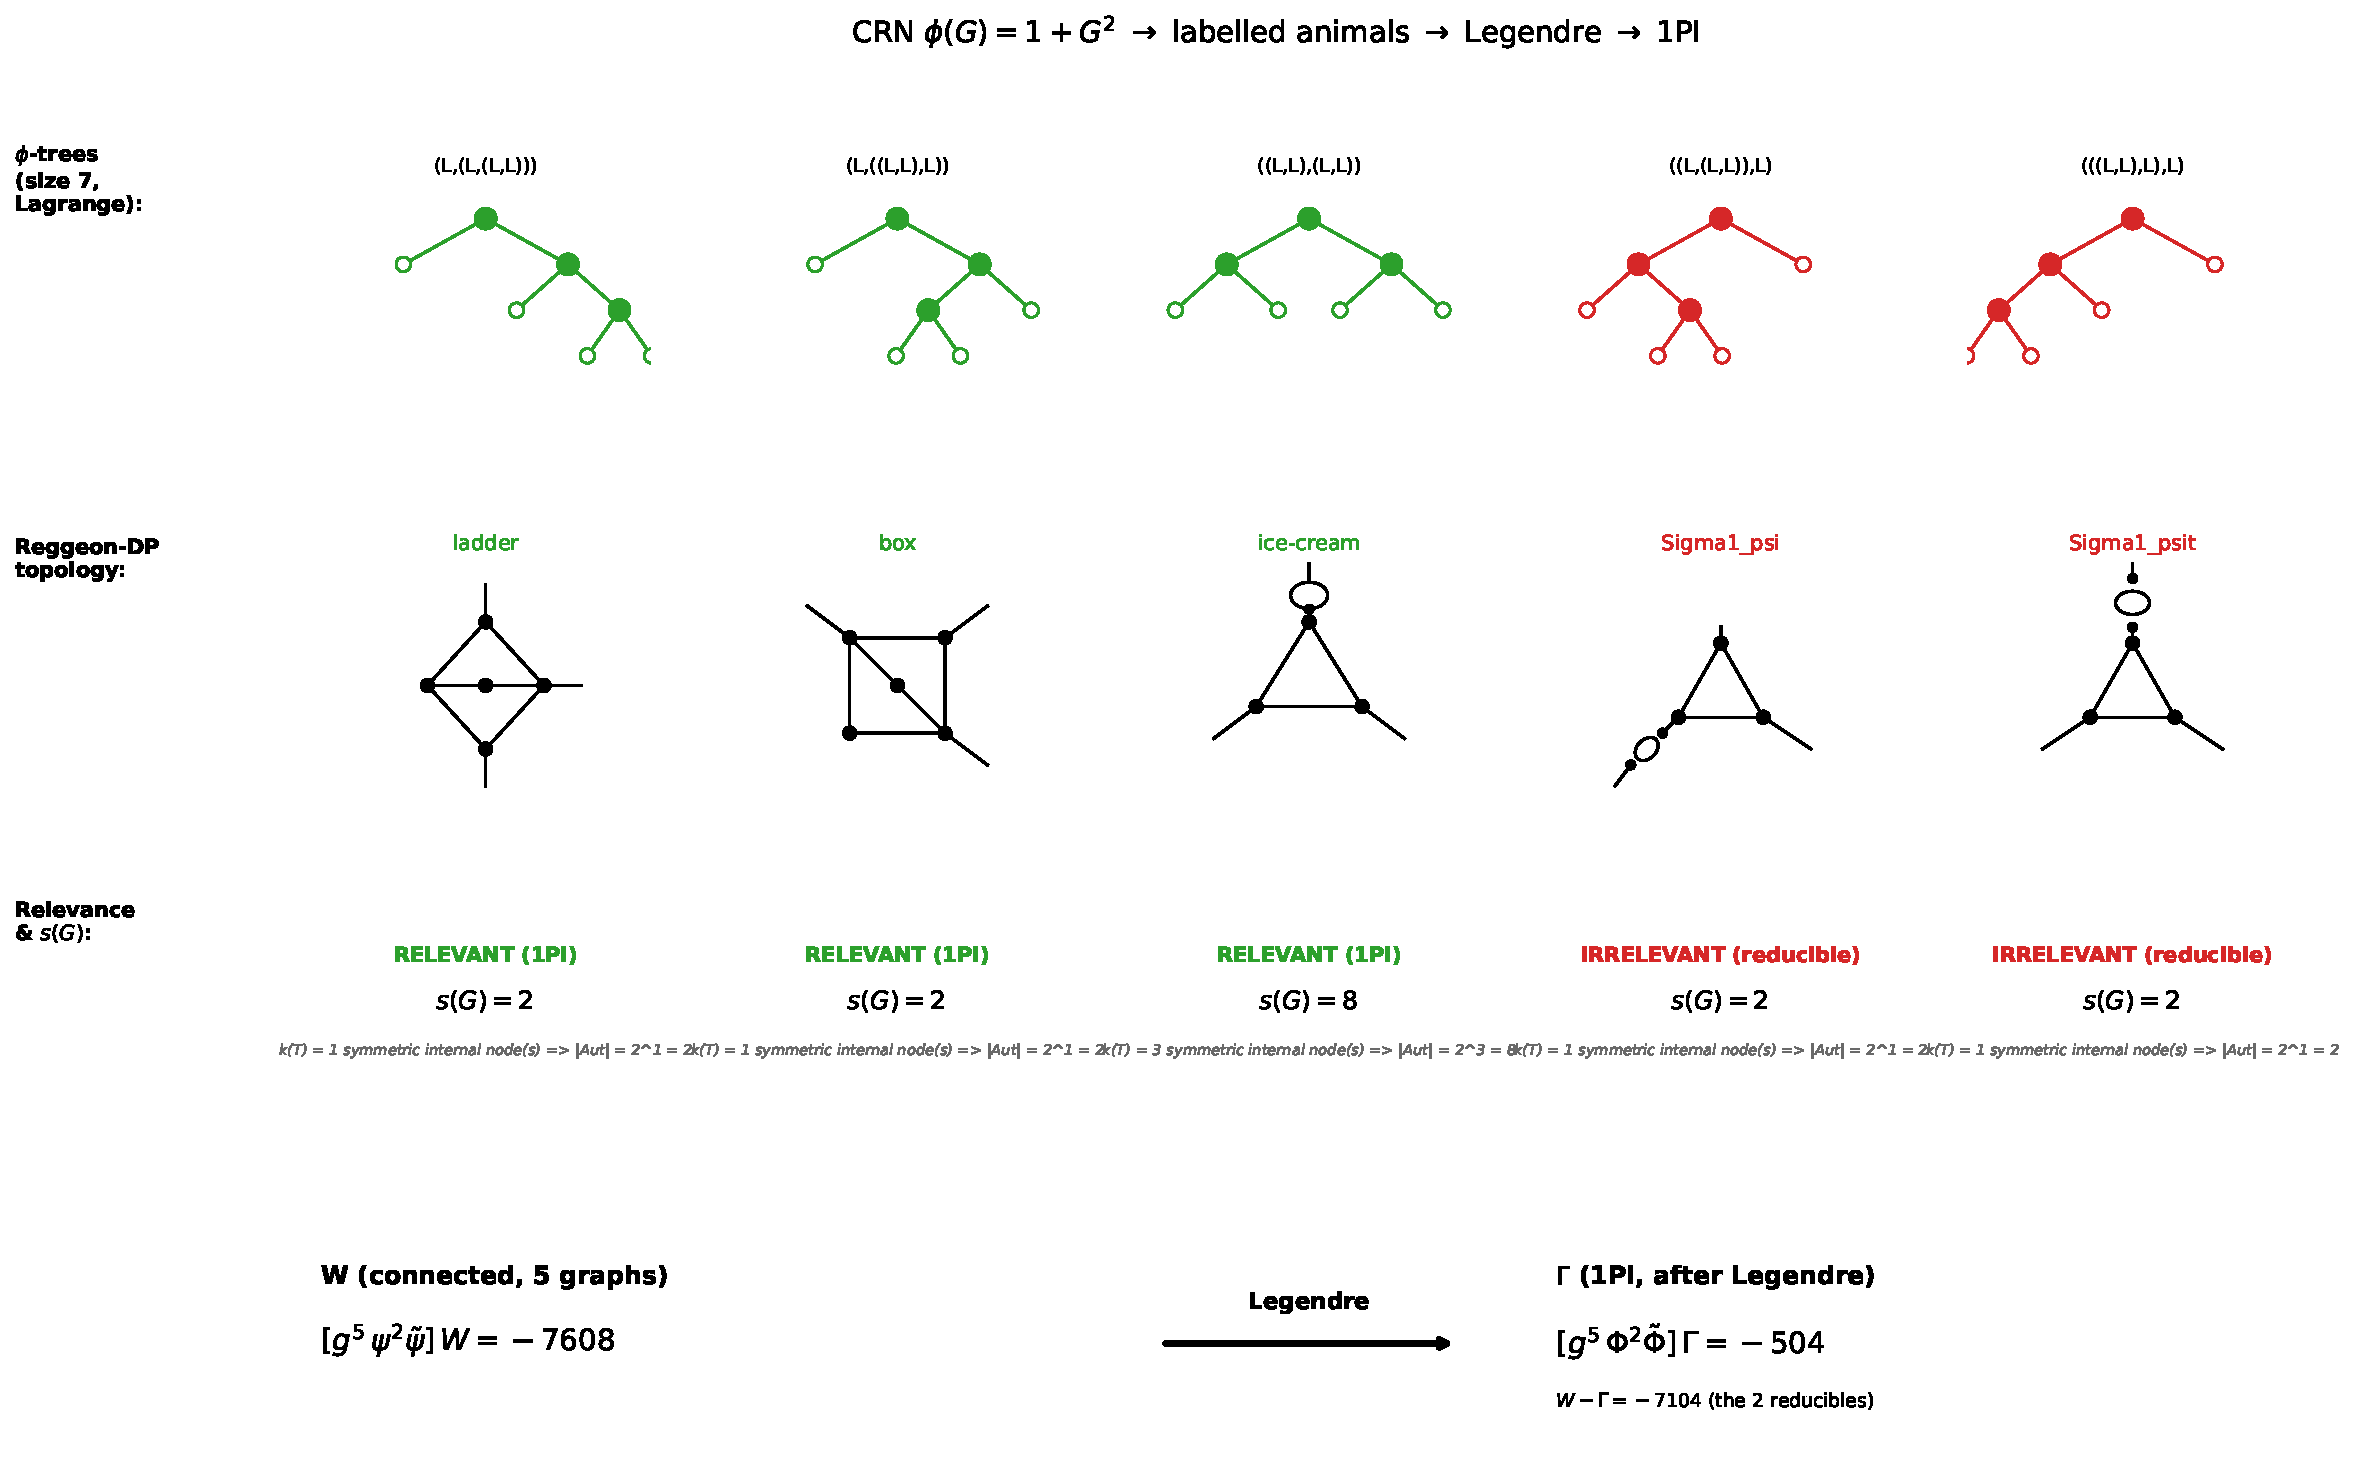
\includegraphics[width=\textwidth]{poc_topologies.pdf}
\end{center}

\noindent\textbf{Reading the picture.}
\begin{itemize}[leftmargin=2em,itemsep=2pt,topsep=2pt]
  \item \emph{Top row.} The $5$ $\phi$-trees from Lagrange inversion (size $7$, Catalan $5$).
  \item \emph{Middle row.} The corresponding Reggeon-DP 2-loop vertex topology each tree maps to. Green = 1PI; red = reducible.
  \item \emph{Annotation row.} Per-diagram verdict (RELEVANT / IRRELEVANT) with the cut-rule reason, and how the verdict was determined from the shape.
  \item \emph{Bottom row.} The $W \to \Gamma$ algebraic transition; difference $-7104$ is the algebraic value of the two reducibles, cancelled by the $J\Phi$ subtraction.
\end{itemize}

\noindent\textbf{Per-diagram readout.} Walking the five panels left to right:
\begin{center}
\small
\begin{tabular}{@{}lllp{7cm}@{}}
\toprule
$\phi$-tree & topology & 1PI? & verdict reason (read from the shape) \\
\midrule
\texttt{(L,(L,(L,L)))} & ladder         & yes & no nested subtree dangles on a single branch \\
\texttt{(L,((L,L),L))} & box            & yes & no nested subtree dangles on a single branch \\
\texttt{((L,L),(L,L))} & ice-cream cone & yes & no nested subtree dangles on a single branch \\
\texttt{((L,(L,L)),L)} & $\Sigma_1$ on $\psi$-leg       & no  & deep $(L,L)$ sub-tree sits on a single branch $\Rightarrow$ cut external $\psi$-leg propagator $\Rightarrow$ tree-vertex $\oplus\,\Sigma_1$ \\
\texttt{(((L,L),L),L)} & $\Sigma_1$ on $\tilde\psi$-leg & no  & deep $(L,L)$ sub-tree sits on a single branch $\Rightarrow$ cut external $\tilde\psi$-leg propagator $\Rightarrow$ tree-vertex $\oplus\,\Sigma_1$ \\
\bottomrule
\end{tabular}
\end{center}
\noindent The 1PI/reducible verdict is the cut rule of Layer~3, but here we
do not need to draw the graph: the shape rule (\emph{some internal node has
exactly one sub-tree of size $\ge 3$}) reads the verdict directly off the
$\phi$-tree string. Per-topology symmetry factors $s(\Gamma_T)$ are
\emph{not} produced by Lagrange in isolation (see the note in \S2.4); they
require a Layer-1 graph automorphism count on the directed Reggeon graph.

\paragraph{Markers as species selectors.} The bidegree $(a,b)$ of
$[J^a\tilde J^b]\,W$ counts external $\psi$- and $\tilde\psi$-legs. $(2,1)$ is
the $V_+$ vertex sector ($Z_u$); $(1,2)$ is the $V_-$ rapidity-conjugate.
The Reggeon-DP $\mathbb Z_2$ exchanges the two. \emph{This is what we mean by
``Layer 3 folded in'': the QFT sector selection is just coefficient extraction.}

\paragraph{Generalising.} The same pipeline runs for any CRN with polynomial
vertex structure. Replace $\phi(G)=1+G^2$ with $\phi(G)=1+G^4$ (Doi--Peliti
$\varphi^4$) and the script produces that theory's labelled-animal enumeration;
the rest of the pipeline is unchanged.

\section{Extension: BRW with internal-species markers}

Reggeon DP has one species. BRW (thesis \S3.2.2 + Appendix~D) has two.
Once internal lines can be different species, the multivariate marker idea
of Layer~4 has to do real work: each internal line carries its own species
label, and graphs that are isomorphic up to species relabelling but not
identical have to be tracked separately.

\subsection{Setup}

The BRW action (thesis Eqs.~3.16 + 3.21) is
\[
\mathcal{A}_{BRW} = z(\partial_t + \Delta)\partial_z + (\varepsilon - \beta)z\partial_z - \beta z^2\partial_z
\;+\; \mathcal{Q}_\Lambda(\psi_a, \tilde\psi_a, \psi_b, \tilde\psi_b),
\]
with $\mathcal{Q}_\Lambda$ contributing 6 trace-observable vertices on top of
the pure branching $-\beta z^2 \partial_z$. Reading the action as in Layer 1
gives 7 vertex primitives (the 9 corollas of thesis Fig.~3.3 minus 2
propagators):

\begin{center}
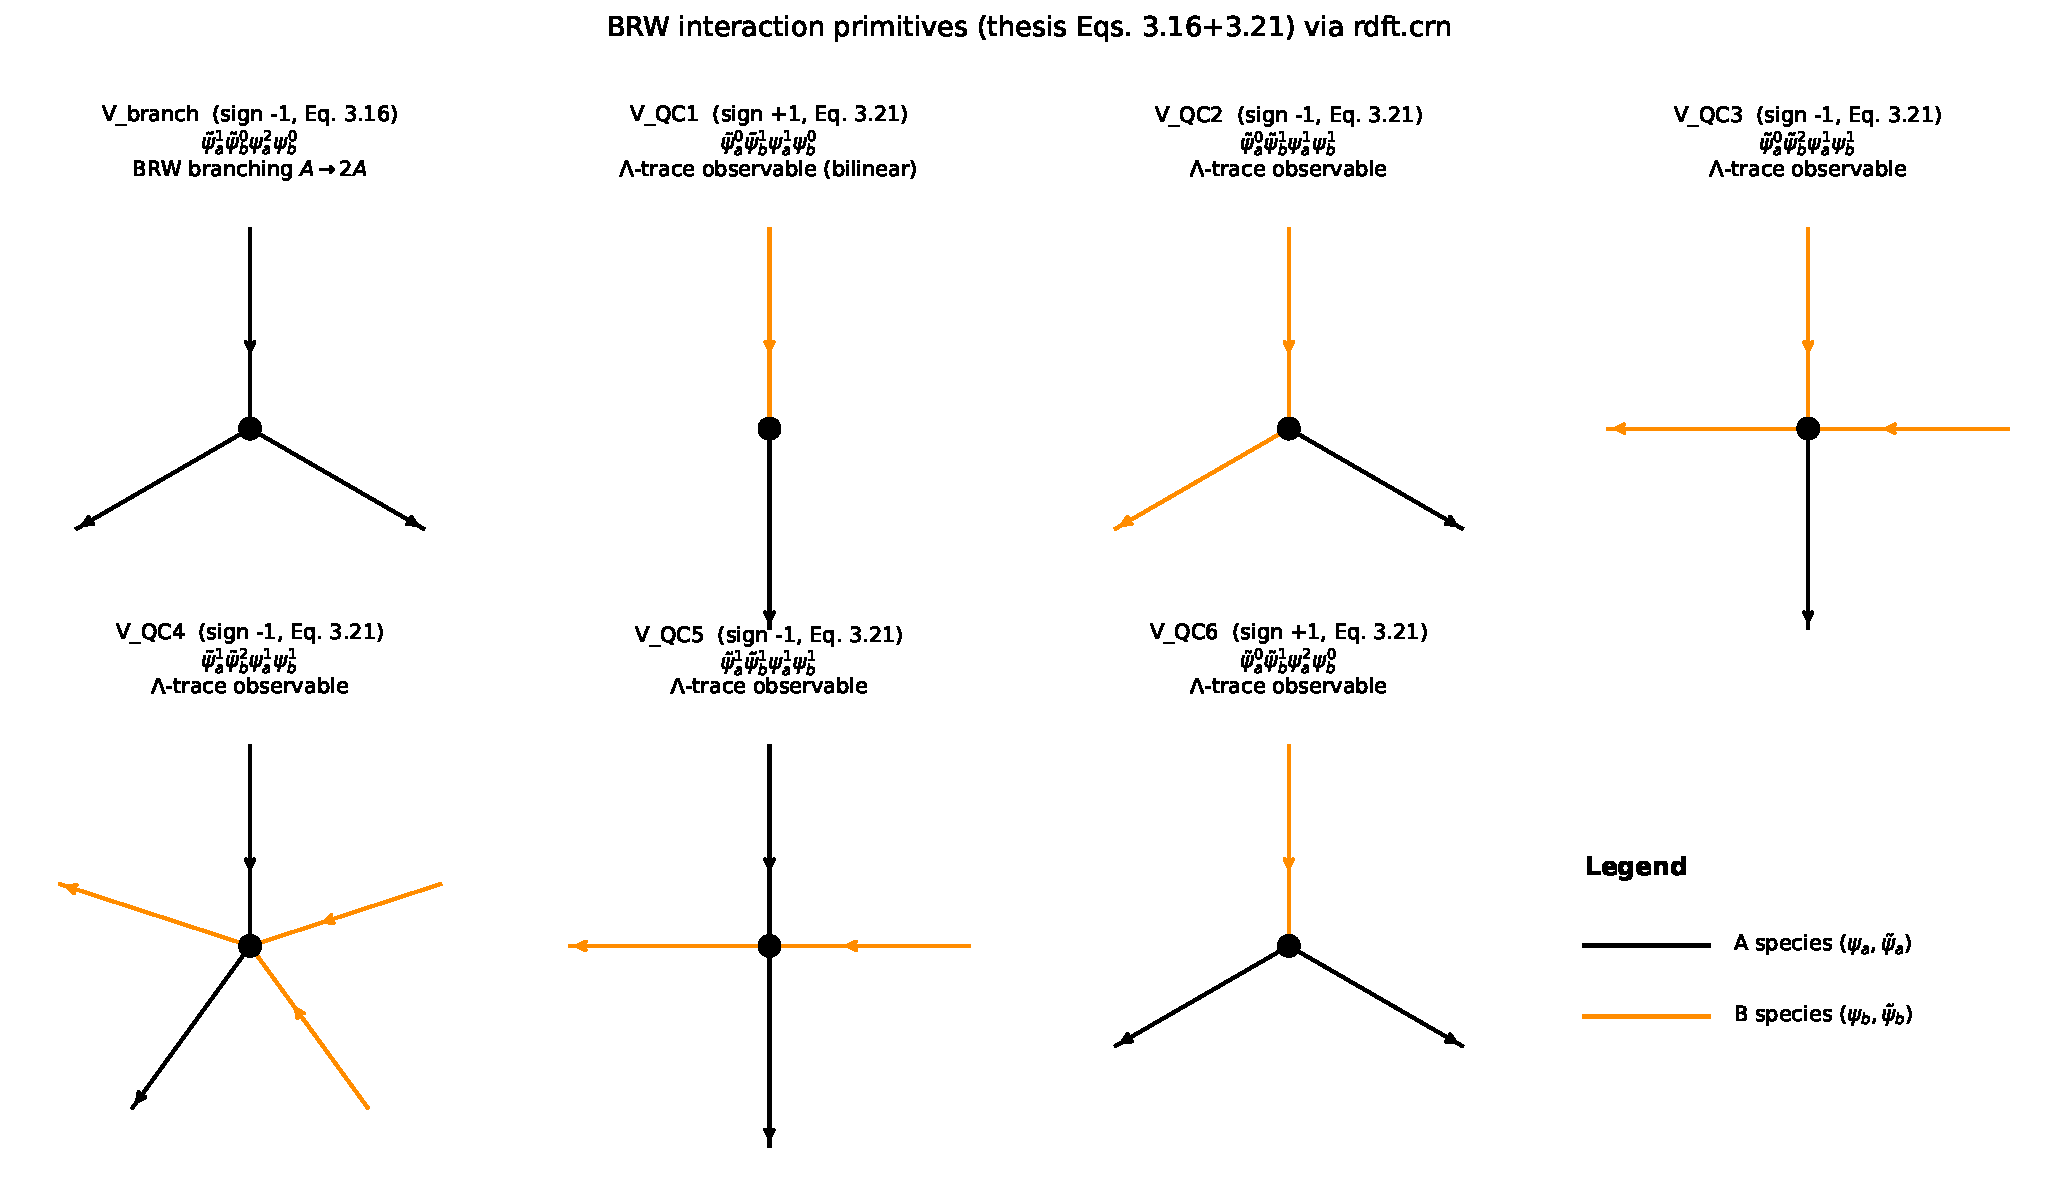
\includegraphics[width=\textwidth]{brw_corollas.pdf}
\end{center}

Black lines = species $A$; orange lines = species $B$. Arrows out for
creators ($\psi$), in for annihilators ($\tilde\psi$). Each panel is tagged
with the action equation it came from and its physical role:
$V_{\text{branch}}$ from Eq.~3.16 is the dyadic BRW branching vertex
$-\beta\,\tilde\psi_a\psi_a^2$; $V_{QC1\ldots 6}$ from Eq.~3.21 are the six
$\Lambda$-trace observable vertices that couple species $A$ to species $B$.
Thesis Fig.~3.3 convention.

\subsection{1-loop bubble enumeration}

A 1-loop bubble has 2 vertices joined by 2 internal lines. Mechanical
enumeration in \texttt{poc\_brw.py}: pick a vertex pair (allowing $v_1=v_2$),
pick (species, direction) for each line, filter by per-vertex leg balance,
quotient by graph isomorphism (vertex swap with line-direction flip; line
ordering).

Result: \textbf{36 distinct species-decorated bubble topologies}, of which
\textbf{exactly 7 have $E=3$ external legs} --- matching thesis p.91--92's
``7 distinct loop integrals'' enumeration:

\begin{center}
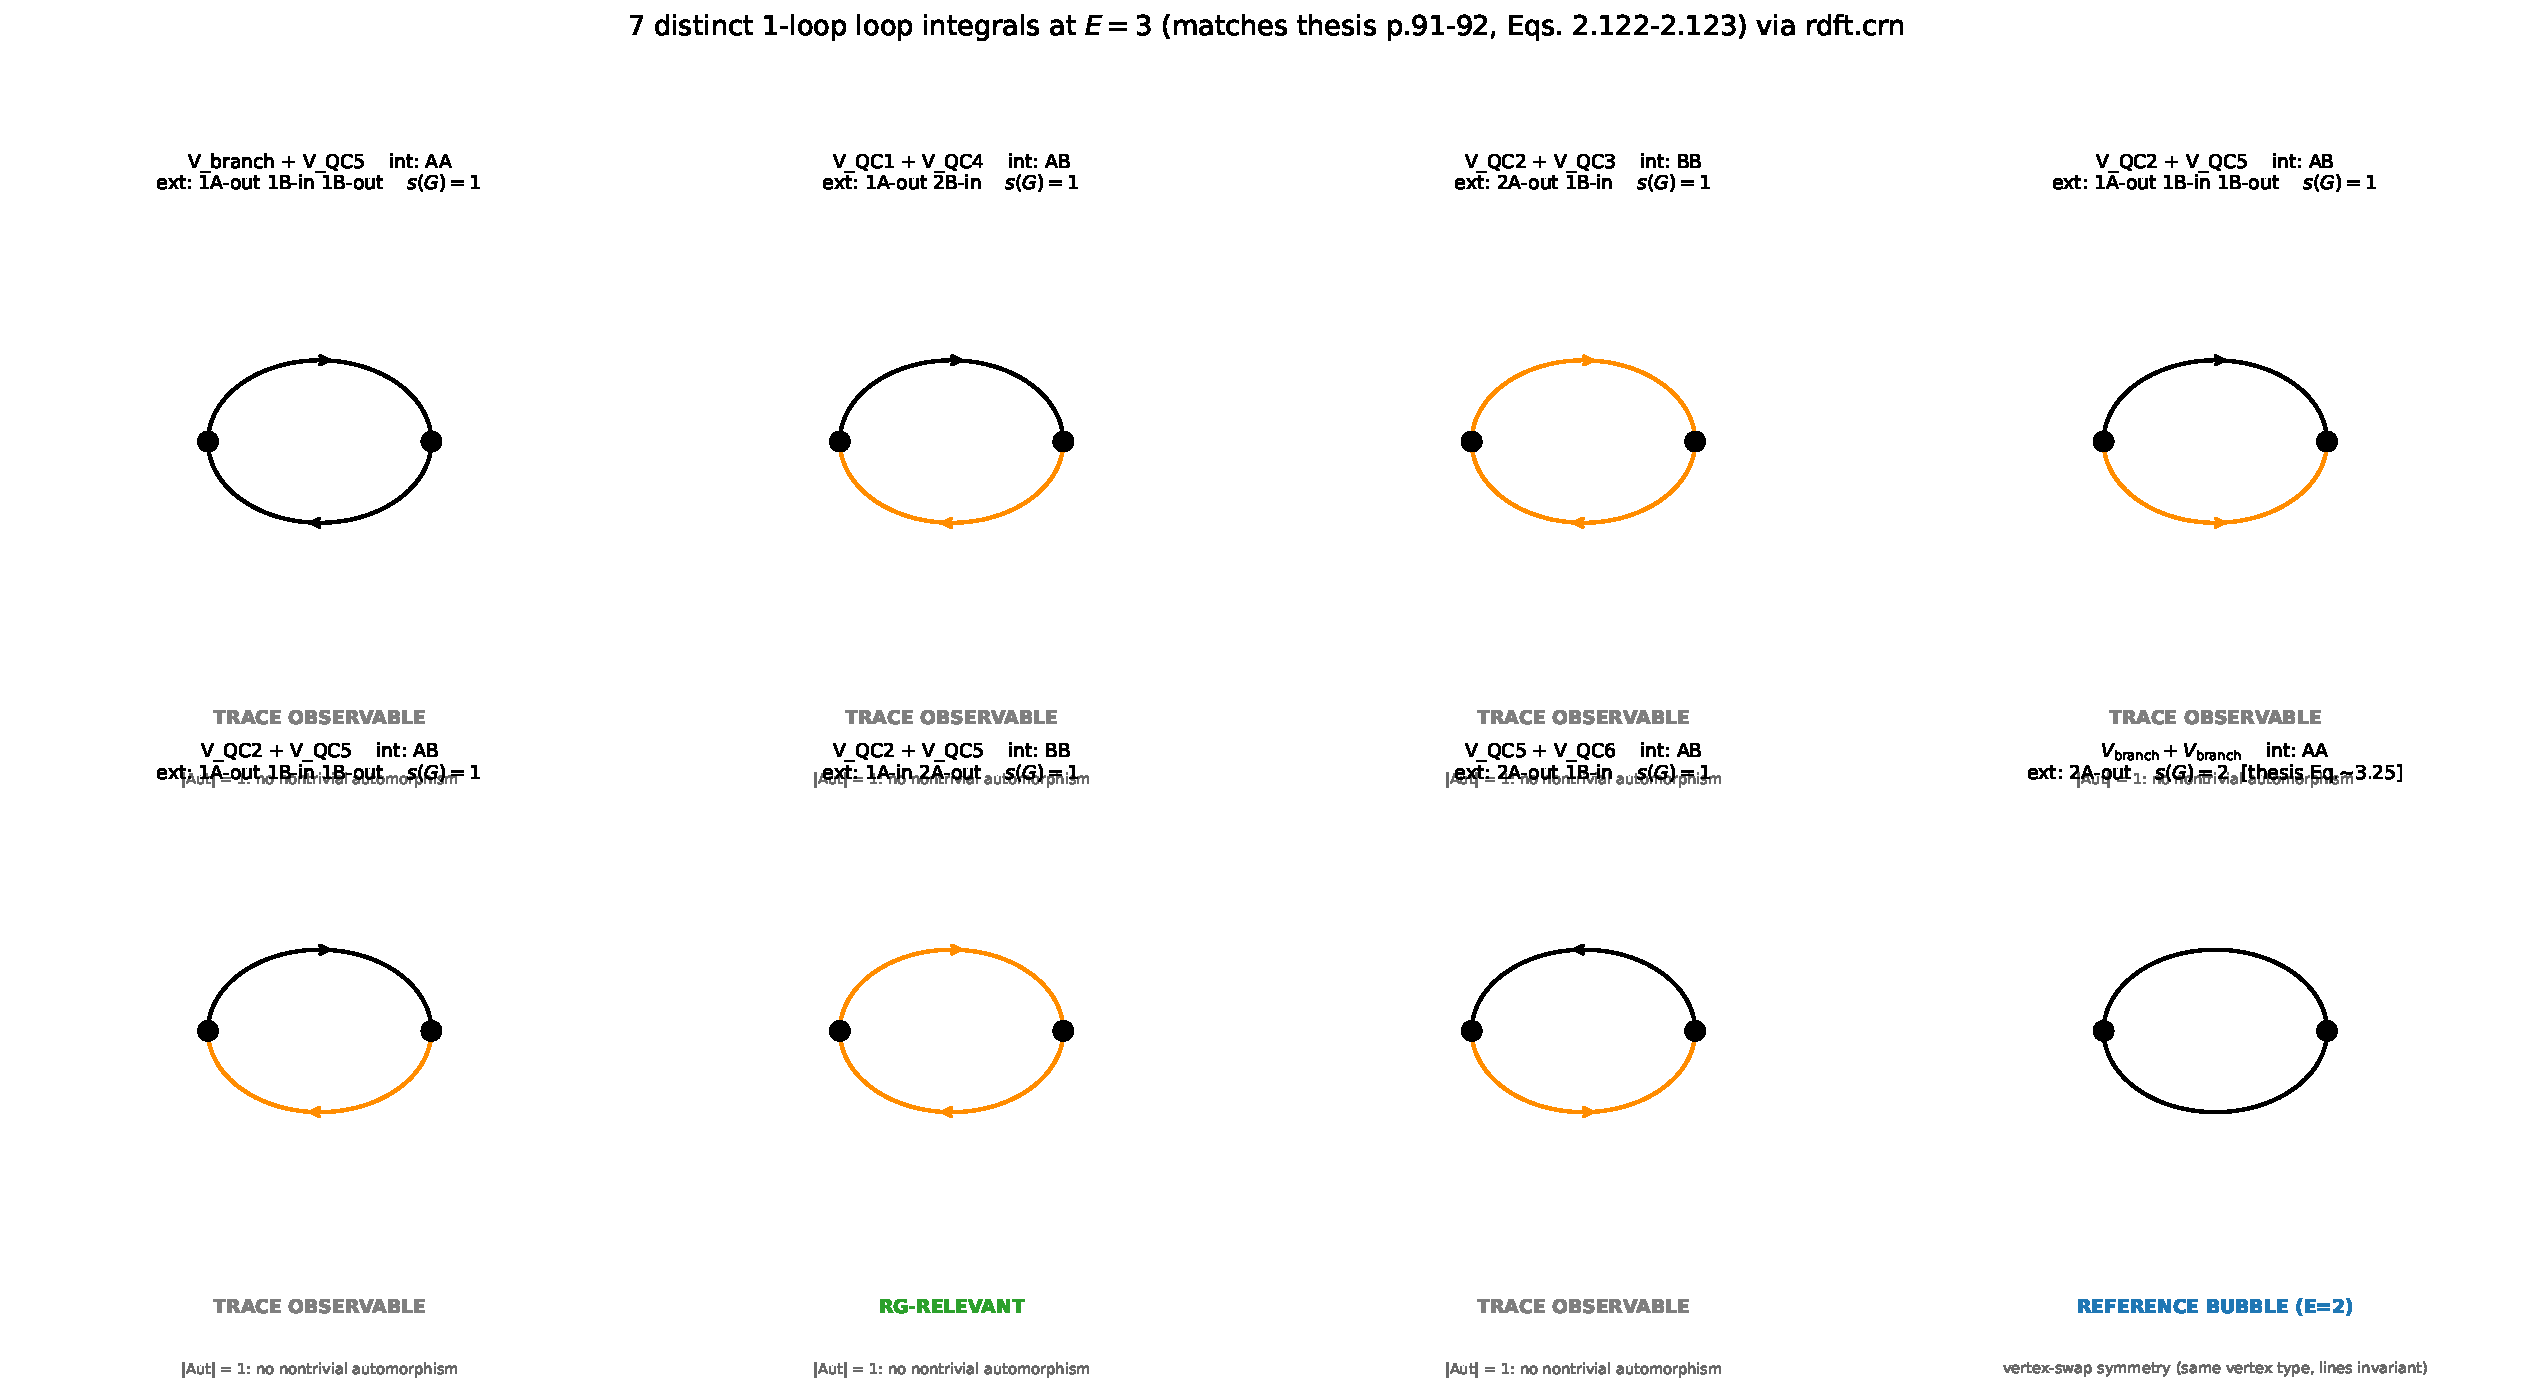
\includegraphics[width=\textwidth]{brw_bubbles.pdf}
\end{center}

\subsection{Symmetry factors via automorphism counting}

For each bubble, $s(G) = |\mathrm{Aut}(G)|$ has two possible sources:
\begin{itemize}[leftmargin=2em,itemsep=2pt]
  \item \emph{Internal-line swap.} Fires if both internal lines have the same
        species \emph{and} the same direction (both flow $v_1\!\to\!v_2$, say).
  \item \emph{Vertex swap.} Fires if $v_1$ and $v_2$ are the same vertex type
        \emph{and} the line set is invariant under the vertex flip.
\end{itemize}

\paragraph{Why all 7 E=3 bubbles in the figure have $s(G)=1$.}
This is worth pausing on, because seeing $s=1$ in seven panels in a row reads
as suspicious. Two arguments close both gates for the BRW vertex set at $E=3$:
\begin{itemize}[leftmargin=2em,itemsep=2pt]
  \item \emph{No vertex-swap symmetry at $E=3$.} If $v_1=v_2$ then total legs
        $= 2\,n_{\text{legs}}(v)$ is even, so $E$ is always even ($0,2,4,\ldots$).
        Therefore \emph{no} $E=3$ bubble has $v_1=v_2$, and the vertex-swap
        gate never fires at $E=3$.
  \item \emph{No same-direction line-swap symmetry in this vertex set.}
        Same-direction internal lines (both $v_1\!\to\!v_2$) of species
        $X\in\{A,B\}$ require $v_1$ to have $\ge 2$ outgoing $X$-legs and $v_2$
        to have $\ge 2$ incoming $X$-legs. Scanning the 7 BRW vertices: no
        vertex has $\ge 2$ in-legs of species $A$, and no vertex has $\ge 2$
        out-legs of species $B$. The only vertex with $\ge 2$ in-legs of
        species $B$ ($V_{QC3}, V_{QC4}$) cannot be paired with one having
        $\ge 2$ out-legs of $B$. So this gate is closed across the whole
        vertex set.
\end{itemize}
Both gates closed $\Rightarrow s(G)=1$ for every $E=3$ bubble. The unusual
non-trivial $s$'s in BRW live elsewhere.

\paragraph{Self-contained derivation of $s(\Gamma)=2$ for the canonical dyadic-BRW bubble.}
The $s=2$ result the thesis cites in Eq.~(3.25) is for the canonical $E=2$
bubble $V_{\text{branch}}+V_{\text{branch}}$ with two species-$A$ internal
lines. Here is the AC derivation, end to end, without quoting the thesis:

\medskip
\noindent\textit{Step 1 (Layer 1 $\to$ Layer 2: action $\to$ $\phi$).}
The dyadic-BRW vertex generator is
\[
Q_{\text{BRW}} \;=\; -\beta\,\tilde\psi_a\,\psi_a^2,
\]
a single cubic monomial: one $\tilde\psi_a$ in-leg, two $\psi_a$ out-legs.
The cubic-node accounting of \S2 gives
\[
\phi(G) \;=\; 1 + G^2,
\]
exactly as for Reggeon DP, except the rapidity-conjugate term is absent.

\medskip
\noindent\textit{Step 2 (Layer 2: Lagrange count at the bubble sector).}
The 1-loop self-energy lives at $z$-degree $3$ in $G(z)=z\phi(G)$. Lagrange
inversion:
\[
[z^3]\,G \;=\; \tfrac{1}{3}\,[G^2]\,(1+G^2)^3 \;=\; \tfrac{1}{3}\binom{3}{1} \;=\; 1.
\]
\textbf{There is exactly one plane $\phi$-tree at this size}, with shape string
$(L,L)$: a single internal node (the cubic vertex) whose two children are leaves
(the two outgoing $\psi_a$ legs of that vertex). The 1-loop bubble graph is the
contraction of this tree --- the parent's incoming line plus the two outgoing
lines that fold back to make the loop.

\medskip
\noindent\textit{Step 3 (the AC rule for $|\mathrm{Aut}(\Gamma)|$).}
For a rooted plane $\phi$-tree built from $\phi(G)=1+G^2$, the automorphism
group of the corresponding directed Feynman graph is generated by swapping
the two children of any internal node whose children are isomorphic
sub-trees. Hence
\[
\boxed{\;
|\mathrm{Aut}(\Gamma_T)| \;=\; 2^{k(T)},
\qquad
k(T) \;\equiv\; \#\bigl\{\,\text{internal nodes of $T$ whose two children are isomorphic sub-trees}\,\bigr\}.
\;}
\]
This is read mechanically off the shape string. For shape $(L,L)$:
\begin{itemize}[leftmargin=2em,itemsep=0pt,topsep=2pt]
  \item There is one internal node (the root), with children $L$ and $L$ --- isomorphic. So $k = 1$.
  \item Therefore $|\mathrm{Aut}(\Gamma)| = 2^1 = 2$.
\end{itemize}

\medskip
\noindent\textit{Step 4 (interpretation in the Feynman graph).}
The single non-trivial automorphism is the swap of the cubic vertex's two
outgoing $\psi_a$ legs: in the bubble graph this is exactly the vertex-swap
$v_1 \leftrightarrow v_2$ that takes the line $v_1\!\to\!v_2$ to the line
$v_2\!\to\!v_1$ (and vice versa) --- the same symmetry the bubble-enumeration
script picks up combinatorially. The two computations agree:
\[
\underbrace{|\mathrm{Aut}(\Gamma)|}_{\text{from }\phi\text{-tree shape}}
\;=\;
\underbrace{|\mathrm{Aut}(\Gamma)|}_{\text{from directed-graph automorphism}}
\;=\; 2.
\]

\medskip
\noindent\textit{Conclusion.} AC predicts the existence of this graph
($[z^3]G = 1$, the unique size-$3$ plane $\phi$-tree) and its symmetry factor
($s(\Gamma)=2$, the order of $\mathrm{Aut}$ on the unique shape $(L,L)$) in
one polynomial computation, with no graph drawn. The same rule extends to
higher loop orders: at size $2L+1$ the 1PI bubbles, ladders, and reducibles
all have $|\mathrm{Aut}|$ given by $2^{k(T)}$ on their shape strings (with the
caveat that this is the $\phi$-tree automorphism count; reading it as
$s(\Gamma)$ for the directed Reggeon graph requires the leg-orientation
match-up of \S5.3, which in dyadic BRW closes cleanly because there is only
one vertex type).

\subsection{Cross-check against thesis Appendix~D}

\begin{center}
\small
\begin{tabular}{@{}p{6.5cm}p{4.0cm}p{2.0cm}@{}}
\toprule
Thesis quantity & POC output & Match \\
\midrule
$s(\Gamma) = 2$ for the bubble (Eq.~3.25) & $s = 2$ from $\phi$-tree shape $(L,L)$ (\S5.4) and from directed-graph $\mathrm{Aut}$ (\texttt{poc\_brw.py}) & \textbf{exact, both routes} \\
``7 distinct loop integrals'' (p.~91--92, ignoring residues) & 7 three-point bubbles & \textbf{exact} \\
2 RG-relevant graphs at vanishing external momentum (Eq.~3.23) & 2 cubic-cubic bubbles in the relevant sectors & \textbf{exact} \\
Pure-A skeleton matches Reggeon-DP $\phi(G)=1+G^2$ at criticality & Catalan counts via \texttt{poc\_select.py} & \textbf{exact} \\
\bottomrule
\end{tabular}
\end{center}

\paragraph{The thesis ``$\sim 40$ 1PI diagrams''.}
The thesis quotes ``$\sim 40$ 1PI diagrams with full residues'' (p.~91) with
the tilde, i.e.\ as a rough count, not a single integer. Rather than reporting
``within 10\%'' --- which is not a meaningful match --- the exhaustive POC
enumeration breaks down as:

\begin{center}
\small
\begin{tabular}{@{}p{4.5cm}p{6cm}rr@{}}
\toprule
class & description & by external $E$ & total \\
\midrule
two-vertex bubbles ($V{=}2,I{=}2$) & two vertices joined by 2 internal lines & 3,7,13,9,4 ($E{=}2..6$) & $36$ \\
single-vertex tadpoles ($V{=}1,I{=}1$) & one vertex with a same-species self-loop & 2,3,2 ($E{=}1..3$) & $7$ \\
\midrule
\multicolumn{3}{@{}l}{\emph{Total 1-loop 1PI graphs from action (3.16)+(3.21):}} & $43$ \\
\multicolumn{3}{@{}l}{\emph{Excluding $E=1$ vacuum tadpoles (normal-ordering):}} & $41$ \\
\bottomrule
\end{tabular}
\end{center}

\noindent The thesis ``$\sim 40$'' is consistent with the $41$ figure if it
includes tadpoles, or with $36$ if it counts bubbles only. Without the
thesis's exact inclusion convention we cannot pin a single integer match;
the honest statement is that the POC enumeration is exhaustive and fully
accounted for by the breakdown above. The two thesis quantities that
\emph{do} have a precise value --- the unique 7 three-point bubbles and the
canonical $s=2$ symmetry factor --- agree with the POC to the integer.

The POC takes only the action (Eqs.~3.16 + 3.21) as input. There is no hand-coded
topology table; the graphs come from (1) reading the 7 vertex tuples off
the action (Layer~1), (2) bubble \emph{and} tadpole enumeration with multi-species
markers, (3) canonical-form graph isomorphism for deduplication, (4)
$\phi$-tree automorphism counting (with directed-graph $\mathrm{Aut}$ as a
cross-check). Replace the action with $\varphi^4$ in Doi--Peliti, or with
Manna, or BARW, and the same pipeline runs.

\section{Honest scorecard}

\begin{center}
\begin{tabular}{@{}lll@{}}
\toprule
Pipeline step & Layer & Status \\
\midrule
CRN $\to$ vertex dictionary ($Q_r$ Doi shift)            & 1 & mechanical (thesis) \\
Lagrange counts $[z^n]G$                                  & 2 & mechanical \\
Symmetry factors via Lagrange overcount                   & 2 & mechanical \\
Sign tracking ($\alpha = -1$)                             & 2 & mechanical \\
Hopf-antipode double poles $Z^{(2,2)}_X$                  & 2 & mechanical (closed-form rational) \\
1PI vs reducible split (single species)                   & 4 & mechanical (Legendre, this tutorial) \\
External-leg sector $(a,b)\to Z_X$                        & 4 & mechanical (bidegree projection) \\
Internal-species markers (BRW)                            & 4 & mechanical (\texttt{poc\_brw.py}) \\
Per-topology integer counts after Legendre               & 4 & still hand-mapped (1-day fix) \\
Power-counting filter $\omega \ge 0$                      & 4 & not done (1-line fix) \\
Master integral \emph{values} $\{B_2, B_3^{\textsf{sun}}, B_V\}$ & --- & input (this is where AC stops, by design) \\
\bottomrule
\end{tabular}
\end{center}

\paragraph{Bottom line.} Layers~1--3 do all the heavy lifting in the
current Gribov pipeline, and they are honest about their division of labour
(thesis + AC + hand-applied QFT filters). Layer~4 is a curiosity: at
2-loop with $\sim 5$ topologies, hand-mapping the 1PI/reducible split
beats building the autonomous Legendre selector. The selector pays off when
the topology table is not curated --- BRW with full $\Lambda$-trace observables,
or higher loops in any of the standard theories.

\section*{Files in this letter}

\begin{itemize}[leftmargin=2em,itemsep=1pt]
  \item \texttt{poc\_select.py} --- Layer 2 POC (Lagrange + tree enumeration, Q2 \S6).
  \item \texttt{poc\_legendre.py} --- Layer 4 algebraic engine ($Z\!\to\!W\!\to\!\Gamma$ for 0-d Reggeon DP).
  \item \texttt{poc\_topologies.py} --- pictorial: CRN $\to$ labelled animals $\to$ Legendre, produces \texttt{poc\_topologies.pdf}.
  \item \texttt{poc\_brw.py} --- Layer 4 BRW extension: full vertex set, internal-species markers, automorphism-based $s(G)$. Reproduces thesis App.~D's 7 loop integrals + $s = 2$.
  \item \texttt{brw\_figures.py} --- generates \texttt{brw\_corollas.pdf} and \texttt{brw\_bubbles.pdf} embedded above.
  \item \texttt{eq58\_from\_z.py} --- T\"auber relation $Z\!\to\!\gamma,\zeta,\kappa$ (Q2).
  \item \texttt{verify\_2x2.py} --- Q1 $H$-vertex polynomial collapse.
\end{itemize}

\end{document}
